% RAG end-to-end pipeline — ingestion + query
% Compile: pdflatex rag_pipeline.tex
% Transparent PNG: gs -sDEVICE=pngalpha -r300 -o rag_pipeline.png rag_pipeline.pdf
\documentclass[tikz,border=12pt]{standalone}
\usepackage{tikz}
\usetikzlibrary{positioning,arrows.meta,shapes.geometric,fit,backgrounds,calc}

\begin{document}
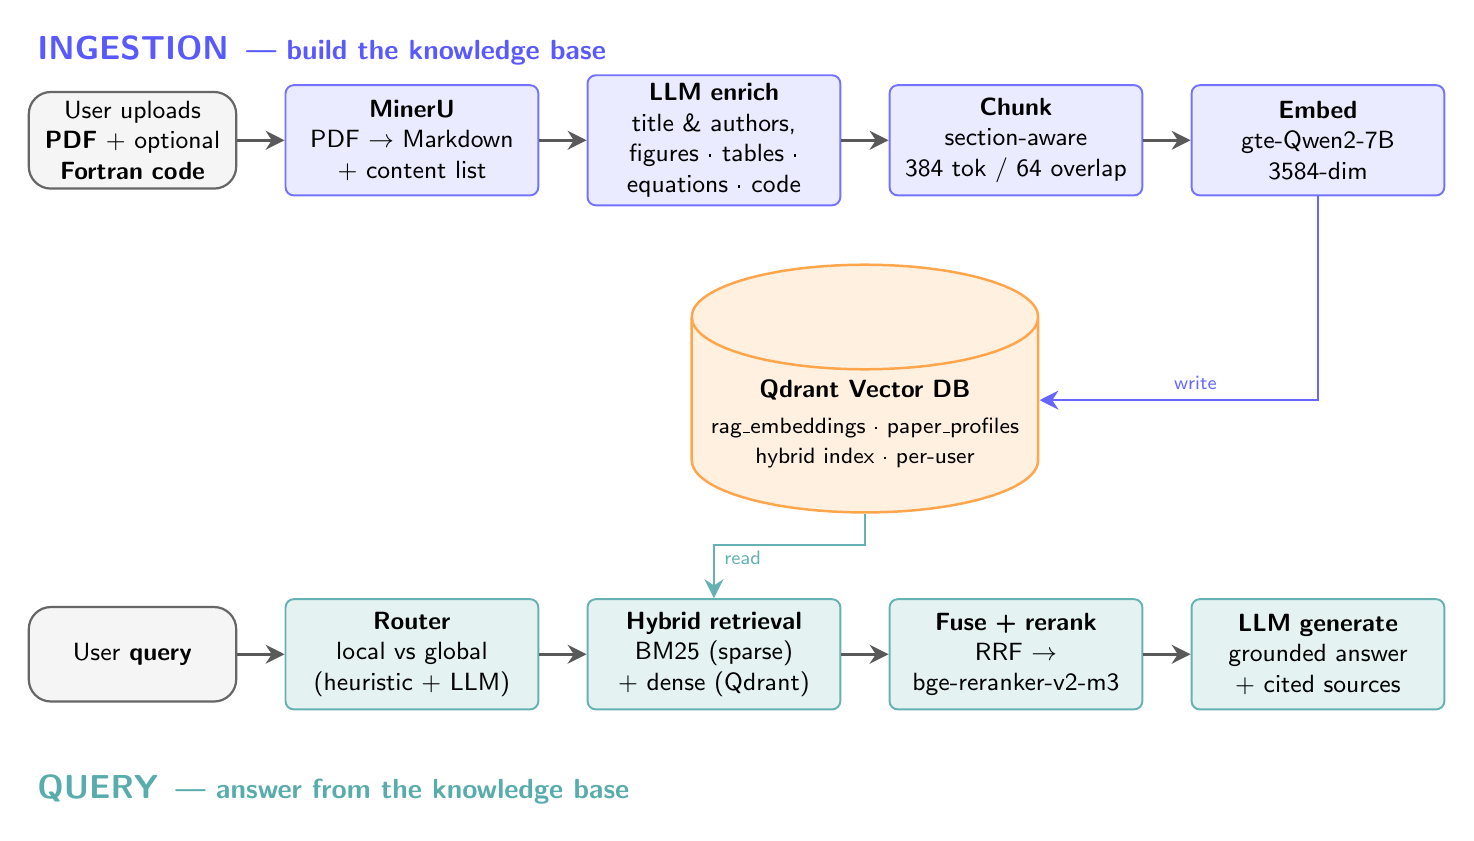
\begin{tikzpicture}[
    font=\sffamily,
    node distance=6mm,
    % ---- styles -------------------------------------------------
    stage/.style={
        rounded corners=3pt, draw=black!55, line width=0.7pt,
        text width=30mm, minimum height=14mm, align=center,
        inner sep=3pt, font=\sffamily\small},
    ingest/.style={stage, fill=blue!8,  draw=blue!55},
    query/.style={stage,  fill=teal!10, draw=teal!60},
    db/.style={
        cylinder, shape border rotate=90, aspect=0.32,
        draw=orange!70, line width=0.9pt, fill=orange!12,
        minimum width=44mm, minimum height=20mm, align=center,
        font=\sffamily\small},
    io/.style={
        rounded corners=8pt, draw=black!60, line width=0.8pt,
        fill=black!4, text width=24mm, minimum height=12mm,
        align=center, font=\sffamily\small},
    flow/.style={-{Stealth[length=2.4mm,width=2.4mm]}, line width=0.9pt, draw=black!65},
    write/.style={flow, draw=blue!60},
    read/.style={flow, draw=teal!60},
    lane/.style={font=\sffamily\bfseries\small, text=black!70},
]

% =================== INGESTION LANE (top) =====================
\node[io]     (upload) {User uploads\\ \textbf{PDF} + optional\\ \textbf{Fortran code}};
\node[ingest, right=of upload] (mineru) {\textbf{MinerU}\\ PDF $\rightarrow$ Markdown\\ + content list};
\node[ingest, right=of mineru] (enrich) {\textbf{LLM enrich}\\ title \& authors,\\ figures · tables ·\\ equations · code};
\node[ingest, right=of enrich] (chunk)  {\textbf{Chunk}\\ section-aware\\ 384 tok / 64 overlap};
\node[ingest, right=of chunk]  (embed)  {\textbf{Embed}\\ gte-Qwen2-7B\\ 3584-dim};

\draw[flow]  (upload) -- (mineru);
\draw[flow]  (mineru) -- (enrich);
\draw[flow]  (enrich) -- (chunk);
\draw[flow]  (chunk)  -- (embed);

% =================== VECTOR DB (centre) =======================
\node[db] (qdrant) at ($(enrich)!0.5!(chunk)+(0,-36mm)$)
    {\textbf{Qdrant Vector DB}\\[2pt] \footnotesize rag\_embeddings · paper\_profiles\\ \footnotesize hybrid index · per-user};

% =================== QUERY LANE (bottom) ======================
\node[io] (ask) at ($(upload.south)+(0,-59mm)$) {User \textbf{query}};
\node[query, right=of ask]     (router)  {\textbf{Router}\\ local vs global\\ (heuristic + LLM)};
\node[query, right=of router]  (retrieve){\textbf{Hybrid retrieval}\\ BM25 (sparse)\\ + dense (Qdrant)};
\node[query, right=of retrieve](rerank)  {\textbf{Fuse + rerank}\\ RRF $\rightarrow$\\ bge-reranker-v2-m3};
\node[query, right=of rerank]  (answer)  {\textbf{LLM generate}\\ grounded answer\\ + cited sources};

\draw[flow]  (ask)     -- (router);
\draw[flow]  (router)  -- (retrieve);
\draw[flow]  (retrieve)-- (rerank);
\draw[flow]  (rerank)  -- (answer);

% =================== DB connections ===========================
\draw[write] (embed.south) |- ([yshift=3mm]qdrant.east)
    node[pos=0.72,above,font=\scriptsize\sffamily,text=blue!60]{write};
\draw[read]  (qdrant.south) -- ++(0,-4mm) -| (retrieve.north)
    node[pos=0.62,right,font=\scriptsize\sffamily,text=teal!60]{read};

% =================== lane labels ==============================
\node[lane, above=2mm of upload.north west, anchor=south west, text=blue!65]
    {\large INGESTION  \normalsize\,— build the knowledge base};
\node[lane, below=8mm of ask.south west, anchor=north west, text=teal!65]
    {\large QUERY  \normalsize\,— answer from the knowledge base};

\end{tikzpicture}
\end{document}
